\section {Pulzní oxymetrie}
\subsection {Historie}
Pulzní oxymetrie je neinvazivní optická technika měření saturace kyslíku v cévách ($SpO_2$). Historie této metody sahá do dob před druhou světovou válkou. Německý lékař a univerzitní profesor Karl Matthes se již od roku 1929, kdy získal doktorát svou prací o zpomalování pulzu morfiem, zabýval oběhovou soustavou. Roku 1935 představil svoji metodu, „\emph{jež umožňuje průběžné zaznamenávání arteriální saturace kyslíkem v lidech způsobem nevyžadujícím krev}". Tuto metodu využíval pro měření plicní kapacity a jako ukazatel metabolického stavu člověka, což však byly v té době již vyřešené problémy. \citep{matthes}
\par Prací na pulzní oxymetrii se však nejvíce proslavil americký fyziolog Glenn Allen Millikan, který vyvinul přístroj fungující na principech Matthesova přístroje, který se připevňoval na ušní lalůček. Pomocí světla průběžně měřil přibližnou saturaci krve kyslíkem u armádních pilotů při letech ve velkých výškách. \citep{TremperPulseOximetry}
\par Tento přístroj, který sloužil jako senzor pro kyslíkovou masku sestával z „\emph{miniaturní žárovky, dvou barevných filtrů a dvou fotočlánků se selenovým přechodem, vážil 30 gramů a nasazoval se přes ucho. Jeden z těchto filtrů propouštěl světlo o vlnové délce, která je stejně pohlcována oxy- a deoxy- hemoglobinem, což zajišťovalo měření celkového množství hemoglobinu v cestě od zdroje světla nehledě na jeho saturaci kyslíkem. Druhá barva byla absorbována těmito dvěma druhy hemoglobinu ve velmi rozdílném množství,}“ díky čemuž se dala dopočítat celková saturace kyslíku v krvi pilota tak, aby kyslíková maska v případě potřeby dodávala správné množství kyslíku. \citep{1942oximeter}
\par Tato převratná metoda se však rozšířila až v 80. letech minulého století, kdy na sálech a jednotkách intenzivní péče doplnila tehdy používanou analýzu parciálního tlaku kyslíku ($PO_2$). Tato metoda se využívala v kombinaci s fyzickými ukazateli, jako například zbarvení kůže do modra, které však kvůli své subjektivitě nebyly vhodné. Ani samo měření $PO_2$ však nebylo optimální metodou - vztah mezi $PO_2$ a saturací kyslíkem totiž není lineární, což znamená, že nebylo snadné výsledky snadno, rychle a správně interpretovat. Kombinace oxymetrie s měřením parciálního tlaku kyslíku přetrvala do současnosti, kdy se pacientovi v anestezii nebo na jednotce intenzivní péče měří saturace průběžnou pulzní oxymetrií v kombinaci s přerušovaným měřením $PO_2$ pomocí analyzátorů krevních plynů. \citep{KYRIACOU}
\begin{figure}[H]
  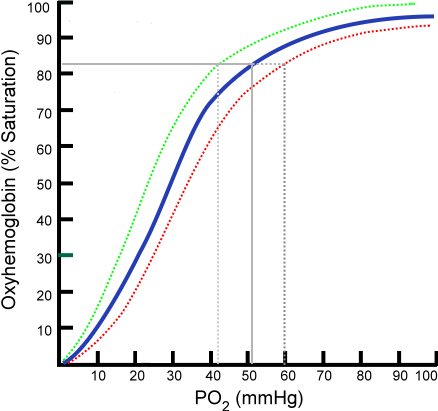
\includegraphics[scale=1, center]{Kapitoly/Teoreticka/Obrazky/TlakKysliku.png}
  \caption [Vztah mezi $PO_2$ a saturací kyslíku v krvi]{Vztah mezi $PO_2$ a saturací kyslíku v krvi, který byl před vynalezením metody pulzní oxymetrie využívaný, není lineární a tudíž nebylo snadné rychle a správně naměřené hodnoty interpretovat. \citep{ratznium_2006}, upraveno}
  \label{fig:PO2}
\end{figure}
\par Pulzní oxymetrie však v současnosti není již specializovanou metodou pro vojenské či zdravotnické účely, ale je používána i v zařízeních určených běžným uživatelům, a to nejen samostatně, ale i jakožto součást komplexnějších produktů. Oproti původnímu Millikanovu oxymetru navíc používáme přesnějších zdrojů světla, LED světlech o specifických vlnových délkách. Zároveň se dá měřit i na jiných částech těla, než je ucho - běžně dostupné oxymetry nejčastěji měří na prstu, existují však i varianty měřící na zápěstí.
\subsection {Princip fungování}
Srdce člověka, jak je obecně známo, funguje v cyklech. Pro krev v tepnách to znamená, že ve chvíli, kdy srdce vypuzuje krev, se zvýší její objem díky elasticitě tepen. Zvýšení tohoto objemu logicky vede k nižší propustnosti světla, díky čemuž mají pulzní oxymetry schopnost měřit srdeční tep.
\par Saturace kyslíku je pak udávána vztahem $SpO_2 = \frac{HbO_2}{\text{Hemoglobin celkem}}$, kde $HbO_2$ je oxyhemoglobin. Tento vztah se pro běžné měření oxymetrem, který umí rozlišovat jen mezi dvěma základními formami hemoglobinu, zjednodušuje na $SpO_2 = \frac{HbO_2}{HbO_2+Hb}$, kde $Hb$ je deoxyhemoglobin). Nové pokročilejší přístroje jsou však schopny detekovat i další formy hemoglobinu - karboxyhemoglobin a methemoglobin. Rovnice pro takovéto měření je pak $SpO_2 = \frac{HbO_2}{HbO_2+Hb+HbCO+HbMet}$, kde $HbCO$ je karboxyhemoglobin a $HbMet$ je methemoglobin. 
\subsubsection{Aplikace Lambertova-Beerova zákona} Samotné měření saturace kyslíku v krvi pak probíhá na principu Lambertova-Beerova zákona, který popisuje pohlcováni elektromagnetické záření. Aplikace tohoto zákona je popsána v následujících rovnicích, které popisuje \cite{KYRIACOU}.
\begin{equation}
  {\epsilon_{\lambda}cl} = A_{\lambda} = ln(T) = ln(\frac{I_s}{I_d})
  \label{EQ:Lambertův–Beerův zákon}
\end{equation}\\
Lambertův–Beerův zákon říká, že vynásobením molární absorpce při vlnové délce $\lambda$ ($\epsilon_{\lambda}$), koncentrace absorpční složky ($c$) a dráhy kterou musí světlo přes danou látku urazit ($l$), vyjde bezrozměrná veličina udávající jak daná látka pohlcuje světlo dané vlnové délky. Tato veličina se nazývá absorbance ($A_{\lambda}$). Její logaritmus udává naopak propustnost světla a nazýváme jej transmitance ($T$). Transmitanci také můžeme vyjádřit jako poměr mezi intenzitou světla které látkou projde při systole a intenzitou světla které látkou projde při diastole ($\frac{I_s}{I_d}$).\\
\begin{equation}
    A_{\lambda} = ln(\frac{I_d+AC_{\lambda}}{I_d})
    \label{EQ:ZAKLAD}
\end{equation}\\
Vzhledem k tomu, že jediné proměnlivé vlastnosti námi sledované látky, v tomto případě prstu, je množství a okysličenost krve, můžeme rozdíl mezi již zmíněnými intenzitami světla při různých stavech oběhového systému označit jako celou střídavou složku ($AC_{\lambda}$). To znamená že, při dané vlnové délce platí vztah $AC_{\lambda} = I_s - I_d$. Využitím tohoto vztahu vznikne rovnice \ref{EQ:ZAKLAD}.\\
\begin{equation}
    A_{\lambda} = ln(\frac{I_d+AC_{\lambda}}{I_d}) = ln(1+\frac{AC_{\lambda}}{I_d}) \simeq \frac{AC_{\lambda}}{I_d}
\end{equation}\\
Jednoduchou úpravou zlomku z rovnice \ref{EQ:ZAKLAD} získáváme logaritmus ve tvaru $ln(1+x)$. Takový logaritmus lze pro hodnoty $x$ blížící se nule zjednodušit jako $ln(1+x)\simeq x$.Vzhledem k tomu, že samotná střídavá složka ($AC_{\lambda}$) je většinou jen 1 - 2 \% celkové intenzity světla a je tedy v porovnání s $I_d$ zanedbatelně malá, můžeme tuto úpravu provést se bez ztráty na přesnosti.\\
\begin{equation}
    A_{\lambda} = \frac{AC_{\lambda}}{I_d} = \frac{AC_{\lambda}}{DC_{\lambda}}
    \label{EQ:DC}
\end{equation}\\
Jak již bylo řečeno, $AC_{\lambda}$ nabývá při měření velmi malých hodnot, díky čemuž můžeme rozdíl mezi průměrnou intenzitou světla, jež prošlo prstem (stálá složka - $DC_{\lambda}$) a již zmíněnými intenzitami světla při různých stavech oběhového systému ($I_s$ a $I_d$) označit za zanedbatelný. Toho také využijeme v rovnici \ref{EQ:DC}.\\
\begin{equation}
    R = \frac{A_{\lambda1}}{A_{\lambda2}} = \frac{(\frac{AC_{\lambda1}}{DC_{\lambda1}})}{(\frac{AC_{\lambda2}}{DC_{\lambda2}})}
    \label{EQ:poměr absorbancí}
\end{equation}\\
Poměr absorbancí ($R$) při dvou vhodných vlnových délkách (jak ukazuje rovnice \ref{EQ:poměr absorbancí}) a empiricky získaná kalibrační křivka se používají pro vypočítání $SpO_2$.\\

\subsubsection{Volba vlnových délek}
 
%\begin{figure}[H]
%  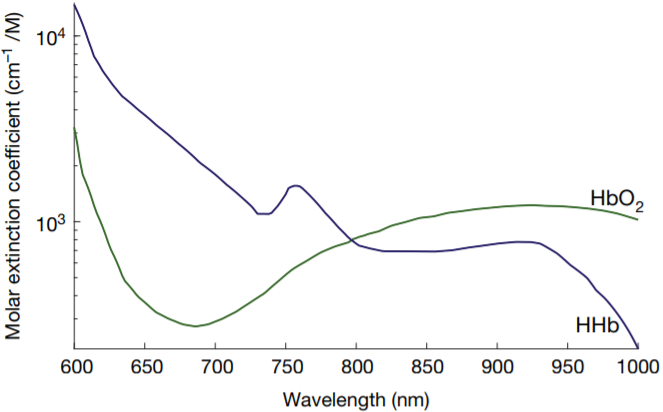
\includegraphics[scale=1, center]{Kapitoly/Teoreticka/Obrazky/Absorpce.png}
%  \caption [Absorpční spektrum HHb a Hb$O_2$]{Absorpční spektrum HHb a Hb$O_2$, na přibližně 805 nanometrech je absorpce stejná, na nižších vlnových délkách absorpci způsobuje převážně HHb, na vyšších pak Hb$O_2$. \citep{KYRIACOU}, upraveno}
%  \label{fig:Absorpce}
%\end{figure}

\subsection {Běžně využívané metody}
Při využívání pulzní oxymetrie jsou 2 různá uspořádání elektroniky využívané pro měření. Jedná se o transmisní a reflektanční měření, která jsou schematicky znázorněna v obrázku \ref{fig:Metody}. Každý z těchto typů měření, jak už jejich názvy napovídají, využívá jiné trajektorie světla skrze prst, což přináší své výhody i nevýhody.
\begin{figure}[H]
    \caption []{}
    \def\svgwidth{\columnwidth}
    \input{Kapitoly/Teoreticka/Obrazky/Metody.pdf_tex}
    \label{fig:Metody}
\end{figure}
\par \textbf{Transmisní metoda} měření spočívá v měření světla, které projde skrz tkáň, což v praxi znamená, že se na kůži z jedné strany svítí oběma diodami a fotodioda se nachází naproti nim. Hlavní výhodou tohoto způsobu měření je vysoká přesnost výsledného měření, které je dosaženo převážně díky přímé trajektorii světla, kdy nezáleží na jeho odrazu od prstu. Naopak hlavní nevýhodou této metody je relativně omezené množství materiálu mezi diodami a fotodiodou, protože při větším množství tkáně v trase světla by již nedocházelo k dostatečnému přenosu světla pro přesné určení saturace. Tato metoda se tedy využívá při měření přes prst, případně ušní lalůček. % Nakreslit obrázek
\par \textbf{Reflektanční metoda} měření naopak využívá světla odraženého tkáněmi pod kůží. To v praxi znamená, že se všechny 3 komponenty (obě LED a fotodioda) nachází na jedné straně ruky (případně jiné části těla), a to tak, že fotodioda se nachází mezi oběma LED, aby se vlivem nerovné vzdálenosti nezkreslovala intenzita záření. Výhodou tohoto měření je, že oxymetr využívající tohoto principu je výrazně přenosnější a pohodlnější pro uživatele, vzhledem k tomu, že ho stačí pouze přiložit. Z tohoto důvodu se využívá ve fitness náramcích a hodinkách, kde by nebylo praktické mít dvě pevné části naproti sobě. Nevýhodou je však nižší přesnost měření, která je převážně důsledkem vysokého rozptylu odraženého světla.